
% Default to the notebook output style

    


% Inherit from the specified cell style.




    
\documentclass[11pt]{article}

    
    
    \usepackage[T1]{fontenc}
    % Nicer default font (+ math font) than Computer Modern for most use cases
    \usepackage{mathpazo}

    % Basic figure setup, for now with no caption control since it's done
    % automatically by Pandoc (which extracts ![](path) syntax from Markdown).
    \usepackage{graphicx}
    % We will generate all images so they have a width \maxwidth. This means
    % that they will get their normal width if they fit onto the page, but
    % are scaled down if they would overflow the margins.
    \makeatletter
    \def\maxwidth{\ifdim\Gin@nat@width>\linewidth\linewidth
    \else\Gin@nat@width\fi}
    \makeatother
    \let\Oldincludegraphics\includegraphics
    % Set max figure width to be 80% of text width, for now hardcoded.
    \renewcommand{\includegraphics}[1]{\Oldincludegraphics[width=.8\maxwidth]{#1}}
    % Ensure that by default, figures have no caption (until we provide a
    % proper Figure object with a Caption API and a way to capture that
    % in the conversion process - todo).
    \usepackage{caption}
    \DeclareCaptionLabelFormat{nolabel}{}
    \captionsetup{labelformat=nolabel}

    \usepackage{adjustbox} % Used to constrain images to a maximum size 
    \usepackage{xcolor} % Allow colors to be defined
    \usepackage{enumerate} % Needed for markdown enumerations to work
    \usepackage{geometry} % Used to adjust the document margins
    \usepackage{amsmath} % Equations
    \usepackage{amssymb} % Equations
    \usepackage{textcomp} % defines textquotesingle
    % Hack from http://tex.stackexchange.com/a/47451/13684:
    \AtBeginDocument{%
        \def\PYZsq{\textquotesingle}% Upright quotes in Pygmentized code
    }
    \usepackage{upquote} % Upright quotes for verbatim code
    \usepackage{eurosym} % defines \euro
    \usepackage[mathletters]{ucs} % Extended unicode (utf-8) support
    \usepackage[utf8x]{inputenc} % Allow utf-8 characters in the tex document
    \usepackage{fancyvrb} % verbatim replacement that allows latex
    \usepackage{grffile} % extends the file name processing of package graphics 
                         % to support a larger range 
    % The hyperref package gives us a pdf with properly built
    % internal navigation ('pdf bookmarks' for the table of contents,
    % internal cross-reference links, web links for URLs, etc.)
    \usepackage{hyperref}
    \usepackage{longtable} % longtable support required by pandoc >1.10
    \usepackage{booktabs}  % table support for pandoc > 1.12.2
    \usepackage[inline]{enumitem} % IRkernel/repr support (it uses the enumerate* environment)
    \usepackage[normalem]{ulem} % ulem is needed to support strikethroughs (\sout)
                                % normalem makes italics be italics, not underlines
    

    
    
    % Colors for the hyperref package
    \definecolor{urlcolor}{rgb}{0,.145,.698}
    \definecolor{linkcolor}{rgb}{.71,0.21,0.01}
    \definecolor{citecolor}{rgb}{.12,.54,.11}

    % ANSI colors
    \definecolor{ansi-black}{HTML}{3E424D}
    \definecolor{ansi-black-intense}{HTML}{282C36}
    \definecolor{ansi-red}{HTML}{E75C58}
    \definecolor{ansi-red-intense}{HTML}{B22B31}
    \definecolor{ansi-green}{HTML}{00A250}
    \definecolor{ansi-green-intense}{HTML}{007427}
    \definecolor{ansi-yellow}{HTML}{DDB62B}
    \definecolor{ansi-yellow-intense}{HTML}{B27D12}
    \definecolor{ansi-blue}{HTML}{208FFB}
    \definecolor{ansi-blue-intense}{HTML}{0065CA}
    \definecolor{ansi-magenta}{HTML}{D160C4}
    \definecolor{ansi-magenta-intense}{HTML}{A03196}
    \definecolor{ansi-cyan}{HTML}{60C6C8}
    \definecolor{ansi-cyan-intense}{HTML}{258F8F}
    \definecolor{ansi-white}{HTML}{C5C1B4}
    \definecolor{ansi-white-intense}{HTML}{A1A6B2}

    % commands and environments needed by pandoc snippets
    % extracted from the output of `pandoc -s`
    \providecommand{\tightlist}{%
      \setlength{\itemsep}{0pt}\setlength{\parskip}{0pt}}
    \DefineVerbatimEnvironment{Highlighting}{Verbatim}{commandchars=\\\{\}}
    % Add ',fontsize=\small' for more characters per line
    \newenvironment{Shaded}{}{}
    \newcommand{\KeywordTok}[1]{\textcolor[rgb]{0.00,0.44,0.13}{\textbf{{#1}}}}
    \newcommand{\DataTypeTok}[1]{\textcolor[rgb]{0.56,0.13,0.00}{{#1}}}
    \newcommand{\DecValTok}[1]{\textcolor[rgb]{0.25,0.63,0.44}{{#1}}}
    \newcommand{\BaseNTok}[1]{\textcolor[rgb]{0.25,0.63,0.44}{{#1}}}
    \newcommand{\FloatTok}[1]{\textcolor[rgb]{0.25,0.63,0.44}{{#1}}}
    \newcommand{\CharTok}[1]{\textcolor[rgb]{0.25,0.44,0.63}{{#1}}}
    \newcommand{\StringTok}[1]{\textcolor[rgb]{0.25,0.44,0.63}{{#1}}}
    \newcommand{\CommentTok}[1]{\textcolor[rgb]{0.38,0.63,0.69}{\textit{{#1}}}}
    \newcommand{\OtherTok}[1]{\textcolor[rgb]{0.00,0.44,0.13}{{#1}}}
    \newcommand{\AlertTok}[1]{\textcolor[rgb]{1.00,0.00,0.00}{\textbf{{#1}}}}
    \newcommand{\FunctionTok}[1]{\textcolor[rgb]{0.02,0.16,0.49}{{#1}}}
    \newcommand{\RegionMarkerTok}[1]{{#1}}
    \newcommand{\ErrorTok}[1]{\textcolor[rgb]{1.00,0.00,0.00}{\textbf{{#1}}}}
    \newcommand{\NormalTok}[1]{{#1}}
    
    % Additional commands for more recent versions of Pandoc
    \newcommand{\ConstantTok}[1]{\textcolor[rgb]{0.53,0.00,0.00}{{#1}}}
    \newcommand{\SpecialCharTok}[1]{\textcolor[rgb]{0.25,0.44,0.63}{{#1}}}
    \newcommand{\VerbatimStringTok}[1]{\textcolor[rgb]{0.25,0.44,0.63}{{#1}}}
    \newcommand{\SpecialStringTok}[1]{\textcolor[rgb]{0.73,0.40,0.53}{{#1}}}
    \newcommand{\ImportTok}[1]{{#1}}
    \newcommand{\DocumentationTok}[1]{\textcolor[rgb]{0.73,0.13,0.13}{\textit{{#1}}}}
    \newcommand{\AnnotationTok}[1]{\textcolor[rgb]{0.38,0.63,0.69}{\textbf{\textit{{#1}}}}}
    \newcommand{\CommentVarTok}[1]{\textcolor[rgb]{0.38,0.63,0.69}{\textbf{\textit{{#1}}}}}
    \newcommand{\VariableTok}[1]{\textcolor[rgb]{0.10,0.09,0.49}{{#1}}}
    \newcommand{\ControlFlowTok}[1]{\textcolor[rgb]{0.00,0.44,0.13}{\textbf{{#1}}}}
    \newcommand{\OperatorTok}[1]{\textcolor[rgb]{0.40,0.40,0.40}{{#1}}}
    \newcommand{\BuiltInTok}[1]{{#1}}
    \newcommand{\ExtensionTok}[1]{{#1}}
    \newcommand{\PreprocessorTok}[1]{\textcolor[rgb]{0.74,0.48,0.00}{{#1}}}
    \newcommand{\AttributeTok}[1]{\textcolor[rgb]{0.49,0.56,0.16}{{#1}}}
    \newcommand{\InformationTok}[1]{\textcolor[rgb]{0.38,0.63,0.69}{\textbf{\textit{{#1}}}}}
    \newcommand{\WarningTok}[1]{\textcolor[rgb]{0.38,0.63,0.69}{\textbf{\textit{{#1}}}}}
    
    
    % Define a nice break command that doesn't care if a line doesn't already
    % exist.
    \def\br{\hspace*{\fill} \\* }
    % Math Jax compatability definitions
    \def\gt{>}
    \def\lt{<}
    % Document parameters
    \title{Homework Week 8}
    
    
    

    % Pygments definitions
    
\makeatletter
\def\PY@reset{\let\PY@it=\relax \let\PY@bf=\relax%
    \let\PY@ul=\relax \let\PY@tc=\relax%
    \let\PY@bc=\relax \let\PY@ff=\relax}
\def\PY@tok#1{\csname PY@tok@#1\endcsname}
\def\PY@toks#1+{\ifx\relax#1\empty\else%
    \PY@tok{#1}\expandafter\PY@toks\fi}
\def\PY@do#1{\PY@bc{\PY@tc{\PY@ul{%
    \PY@it{\PY@bf{\PY@ff{#1}}}}}}}
\def\PY#1#2{\PY@reset\PY@toks#1+\relax+\PY@do{#2}}

\expandafter\def\csname PY@tok@w\endcsname{\def\PY@tc##1{\textcolor[rgb]{0.73,0.73,0.73}{##1}}}
\expandafter\def\csname PY@tok@c\endcsname{\let\PY@it=\textit\def\PY@tc##1{\textcolor[rgb]{0.25,0.50,0.50}{##1}}}
\expandafter\def\csname PY@tok@cp\endcsname{\def\PY@tc##1{\textcolor[rgb]{0.74,0.48,0.00}{##1}}}
\expandafter\def\csname PY@tok@k\endcsname{\let\PY@bf=\textbf\def\PY@tc##1{\textcolor[rgb]{0.00,0.50,0.00}{##1}}}
\expandafter\def\csname PY@tok@kp\endcsname{\def\PY@tc##1{\textcolor[rgb]{0.00,0.50,0.00}{##1}}}
\expandafter\def\csname PY@tok@kt\endcsname{\def\PY@tc##1{\textcolor[rgb]{0.69,0.00,0.25}{##1}}}
\expandafter\def\csname PY@tok@o\endcsname{\def\PY@tc##1{\textcolor[rgb]{0.40,0.40,0.40}{##1}}}
\expandafter\def\csname PY@tok@ow\endcsname{\let\PY@bf=\textbf\def\PY@tc##1{\textcolor[rgb]{0.67,0.13,1.00}{##1}}}
\expandafter\def\csname PY@tok@nb\endcsname{\def\PY@tc##1{\textcolor[rgb]{0.00,0.50,0.00}{##1}}}
\expandafter\def\csname PY@tok@nf\endcsname{\def\PY@tc##1{\textcolor[rgb]{0.00,0.00,1.00}{##1}}}
\expandafter\def\csname PY@tok@nc\endcsname{\let\PY@bf=\textbf\def\PY@tc##1{\textcolor[rgb]{0.00,0.00,1.00}{##1}}}
\expandafter\def\csname PY@tok@nn\endcsname{\let\PY@bf=\textbf\def\PY@tc##1{\textcolor[rgb]{0.00,0.00,1.00}{##1}}}
\expandafter\def\csname PY@tok@ne\endcsname{\let\PY@bf=\textbf\def\PY@tc##1{\textcolor[rgb]{0.82,0.25,0.23}{##1}}}
\expandafter\def\csname PY@tok@nv\endcsname{\def\PY@tc##1{\textcolor[rgb]{0.10,0.09,0.49}{##1}}}
\expandafter\def\csname PY@tok@no\endcsname{\def\PY@tc##1{\textcolor[rgb]{0.53,0.00,0.00}{##1}}}
\expandafter\def\csname PY@tok@nl\endcsname{\def\PY@tc##1{\textcolor[rgb]{0.63,0.63,0.00}{##1}}}
\expandafter\def\csname PY@tok@ni\endcsname{\let\PY@bf=\textbf\def\PY@tc##1{\textcolor[rgb]{0.60,0.60,0.60}{##1}}}
\expandafter\def\csname PY@tok@na\endcsname{\def\PY@tc##1{\textcolor[rgb]{0.49,0.56,0.16}{##1}}}
\expandafter\def\csname PY@tok@nt\endcsname{\let\PY@bf=\textbf\def\PY@tc##1{\textcolor[rgb]{0.00,0.50,0.00}{##1}}}
\expandafter\def\csname PY@tok@nd\endcsname{\def\PY@tc##1{\textcolor[rgb]{0.67,0.13,1.00}{##1}}}
\expandafter\def\csname PY@tok@s\endcsname{\def\PY@tc##1{\textcolor[rgb]{0.73,0.13,0.13}{##1}}}
\expandafter\def\csname PY@tok@sd\endcsname{\let\PY@it=\textit\def\PY@tc##1{\textcolor[rgb]{0.73,0.13,0.13}{##1}}}
\expandafter\def\csname PY@tok@si\endcsname{\let\PY@bf=\textbf\def\PY@tc##1{\textcolor[rgb]{0.73,0.40,0.53}{##1}}}
\expandafter\def\csname PY@tok@se\endcsname{\let\PY@bf=\textbf\def\PY@tc##1{\textcolor[rgb]{0.73,0.40,0.13}{##1}}}
\expandafter\def\csname PY@tok@sr\endcsname{\def\PY@tc##1{\textcolor[rgb]{0.73,0.40,0.53}{##1}}}
\expandafter\def\csname PY@tok@ss\endcsname{\def\PY@tc##1{\textcolor[rgb]{0.10,0.09,0.49}{##1}}}
\expandafter\def\csname PY@tok@sx\endcsname{\def\PY@tc##1{\textcolor[rgb]{0.00,0.50,0.00}{##1}}}
\expandafter\def\csname PY@tok@m\endcsname{\def\PY@tc##1{\textcolor[rgb]{0.40,0.40,0.40}{##1}}}
\expandafter\def\csname PY@tok@gh\endcsname{\let\PY@bf=\textbf\def\PY@tc##1{\textcolor[rgb]{0.00,0.00,0.50}{##1}}}
\expandafter\def\csname PY@tok@gu\endcsname{\let\PY@bf=\textbf\def\PY@tc##1{\textcolor[rgb]{0.50,0.00,0.50}{##1}}}
\expandafter\def\csname PY@tok@gd\endcsname{\def\PY@tc##1{\textcolor[rgb]{0.63,0.00,0.00}{##1}}}
\expandafter\def\csname PY@tok@gi\endcsname{\def\PY@tc##1{\textcolor[rgb]{0.00,0.63,0.00}{##1}}}
\expandafter\def\csname PY@tok@gr\endcsname{\def\PY@tc##1{\textcolor[rgb]{1.00,0.00,0.00}{##1}}}
\expandafter\def\csname PY@tok@ge\endcsname{\let\PY@it=\textit}
\expandafter\def\csname PY@tok@gs\endcsname{\let\PY@bf=\textbf}
\expandafter\def\csname PY@tok@gp\endcsname{\let\PY@bf=\textbf\def\PY@tc##1{\textcolor[rgb]{0.00,0.00,0.50}{##1}}}
\expandafter\def\csname PY@tok@go\endcsname{\def\PY@tc##1{\textcolor[rgb]{0.53,0.53,0.53}{##1}}}
\expandafter\def\csname PY@tok@gt\endcsname{\def\PY@tc##1{\textcolor[rgb]{0.00,0.27,0.87}{##1}}}
\expandafter\def\csname PY@tok@err\endcsname{\def\PY@bc##1{\setlength{\fboxsep}{0pt}\fcolorbox[rgb]{1.00,0.00,0.00}{1,1,1}{\strut ##1}}}
\expandafter\def\csname PY@tok@kc\endcsname{\let\PY@bf=\textbf\def\PY@tc##1{\textcolor[rgb]{0.00,0.50,0.00}{##1}}}
\expandafter\def\csname PY@tok@kd\endcsname{\let\PY@bf=\textbf\def\PY@tc##1{\textcolor[rgb]{0.00,0.50,0.00}{##1}}}
\expandafter\def\csname PY@tok@kn\endcsname{\let\PY@bf=\textbf\def\PY@tc##1{\textcolor[rgb]{0.00,0.50,0.00}{##1}}}
\expandafter\def\csname PY@tok@kr\endcsname{\let\PY@bf=\textbf\def\PY@tc##1{\textcolor[rgb]{0.00,0.50,0.00}{##1}}}
\expandafter\def\csname PY@tok@bp\endcsname{\def\PY@tc##1{\textcolor[rgb]{0.00,0.50,0.00}{##1}}}
\expandafter\def\csname PY@tok@fm\endcsname{\def\PY@tc##1{\textcolor[rgb]{0.00,0.00,1.00}{##1}}}
\expandafter\def\csname PY@tok@vc\endcsname{\def\PY@tc##1{\textcolor[rgb]{0.10,0.09,0.49}{##1}}}
\expandafter\def\csname PY@tok@vg\endcsname{\def\PY@tc##1{\textcolor[rgb]{0.10,0.09,0.49}{##1}}}
\expandafter\def\csname PY@tok@vi\endcsname{\def\PY@tc##1{\textcolor[rgb]{0.10,0.09,0.49}{##1}}}
\expandafter\def\csname PY@tok@vm\endcsname{\def\PY@tc##1{\textcolor[rgb]{0.10,0.09,0.49}{##1}}}
\expandafter\def\csname PY@tok@sa\endcsname{\def\PY@tc##1{\textcolor[rgb]{0.73,0.13,0.13}{##1}}}
\expandafter\def\csname PY@tok@sb\endcsname{\def\PY@tc##1{\textcolor[rgb]{0.73,0.13,0.13}{##1}}}
\expandafter\def\csname PY@tok@sc\endcsname{\def\PY@tc##1{\textcolor[rgb]{0.73,0.13,0.13}{##1}}}
\expandafter\def\csname PY@tok@dl\endcsname{\def\PY@tc##1{\textcolor[rgb]{0.73,0.13,0.13}{##1}}}
\expandafter\def\csname PY@tok@s2\endcsname{\def\PY@tc##1{\textcolor[rgb]{0.73,0.13,0.13}{##1}}}
\expandafter\def\csname PY@tok@sh\endcsname{\def\PY@tc##1{\textcolor[rgb]{0.73,0.13,0.13}{##1}}}
\expandafter\def\csname PY@tok@s1\endcsname{\def\PY@tc##1{\textcolor[rgb]{0.73,0.13,0.13}{##1}}}
\expandafter\def\csname PY@tok@mb\endcsname{\def\PY@tc##1{\textcolor[rgb]{0.40,0.40,0.40}{##1}}}
\expandafter\def\csname PY@tok@mf\endcsname{\def\PY@tc##1{\textcolor[rgb]{0.40,0.40,0.40}{##1}}}
\expandafter\def\csname PY@tok@mh\endcsname{\def\PY@tc##1{\textcolor[rgb]{0.40,0.40,0.40}{##1}}}
\expandafter\def\csname PY@tok@mi\endcsname{\def\PY@tc##1{\textcolor[rgb]{0.40,0.40,0.40}{##1}}}
\expandafter\def\csname PY@tok@il\endcsname{\def\PY@tc##1{\textcolor[rgb]{0.40,0.40,0.40}{##1}}}
\expandafter\def\csname PY@tok@mo\endcsname{\def\PY@tc##1{\textcolor[rgb]{0.40,0.40,0.40}{##1}}}
\expandafter\def\csname PY@tok@ch\endcsname{\let\PY@it=\textit\def\PY@tc##1{\textcolor[rgb]{0.25,0.50,0.50}{##1}}}
\expandafter\def\csname PY@tok@cm\endcsname{\let\PY@it=\textit\def\PY@tc##1{\textcolor[rgb]{0.25,0.50,0.50}{##1}}}
\expandafter\def\csname PY@tok@cpf\endcsname{\let\PY@it=\textit\def\PY@tc##1{\textcolor[rgb]{0.25,0.50,0.50}{##1}}}
\expandafter\def\csname PY@tok@c1\endcsname{\let\PY@it=\textit\def\PY@tc##1{\textcolor[rgb]{0.25,0.50,0.50}{##1}}}
\expandafter\def\csname PY@tok@cs\endcsname{\let\PY@it=\textit\def\PY@tc##1{\textcolor[rgb]{0.25,0.50,0.50}{##1}}}

\def\PYZbs{\char`\\}
\def\PYZus{\char`\_}
\def\PYZob{\char`\{}
\def\PYZcb{\char`\}}
\def\PYZca{\char`\^}
\def\PYZam{\char`\&}
\def\PYZlt{\char`\<}
\def\PYZgt{\char`\>}
\def\PYZsh{\char`\#}
\def\PYZpc{\char`\%}
\def\PYZdl{\char`\$}
\def\PYZhy{\char`\-}
\def\PYZsq{\char`\'}
\def\PYZdq{\char`\"}
\def\PYZti{\char`\~}
% for compatibility with earlier versions
\def\PYZat{@}
\def\PYZlb{[}
\def\PYZrb{]}
\makeatother


    % Exact colors from NB
    \definecolor{incolor}{rgb}{0.0, 0.0, 0.5}
    \definecolor{outcolor}{rgb}{0.545, 0.0, 0.0}



    
    % Prevent overflowing lines due to hard-to-break entities
    \sloppy 
    % Setup hyperref package
    \hypersetup{
      breaklinks=true,  % so long urls are correctly broken across lines
      colorlinks=true,
      urlcolor=urlcolor,
      linkcolor=linkcolor,
      citecolor=citecolor,
      }
    % Slightly bigger margins than the latex defaults
    
    \geometry{verbose,tmargin=1in,bmargin=1in,lmargin=1in,rmargin=1in}
    
    

    \begin{document}
    
    
    \maketitle
    
    

    
    \hypertarget{homework-week-8}{%
\section{Homework Week 8}\label{homework-week-8}}

For each of the following questions please show that the statistical
assumptions for each of the respective tests are met. It is good
practice always before start using statistical analysis to do
descriptive statistics to understand you data. It is not required to
show descriptive analysis here unless there is something important to
report (transformations, deviation from normality, outliers, etc).

    \begin{enumerate}
\def\labelenumi{\arabic{enumi}.}
\tightlist
\item
  The data in the table give the infant mortality rates per 1000
  livebirths in the United States for the period 1960-2000
\end{enumerate}

\begin{figure}
\centering
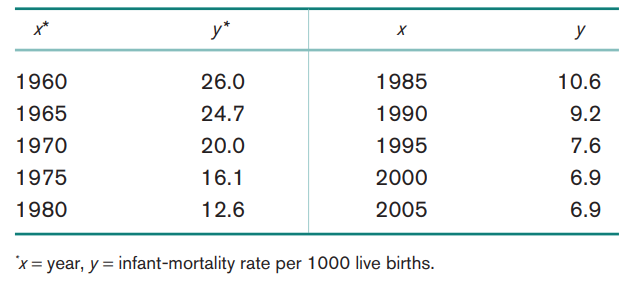
\includegraphics{HW1.png}
\caption{title}
\end{figure}

\begin{enumerate}
\def\labelenumi{\alph{enumi}.}
\item
  Fit a linear regression line relating infant mortality rate to
  chronological year using these data. Use a data transformation if
  necessary
\item
  Test for significance of the linear relationship
\item
  If the present trend continues for the next 5 years what would be the
  predicted infant mortality rate in 2010
\end{enumerate}

    \begin{Verbatim}[commandchars=\\\{\}]
{\color{incolor}In [{\color{incolor}1}]:} \PY{c+c1}{\PYZsh{}from the table above, we have the data from 1960 to 2005 of infant motality per 1000 livebirths:}
        \PY{l+s}{\PYZsq{}}\PY{l+s}{a\PYZsq{}}
        \PY{c+c1}{\PYZsh{}we have x values:}
        x\PY{o}{\PYZlt{}\PYZhy{}}\PY{k+kt}{c}\PY{p}{(}\PY{l+m}{1960}\PY{p}{,}\PY{l+m}{1965}\PY{p}{,}\PY{l+m}{1970}\PY{p}{,}\PY{l+m}{1975}\PY{p}{,}\PY{l+m}{1980}\PY{p}{,}\PY{l+m}{1985}\PY{p}{,}\PY{l+m}{1990}\PY{p}{,}\PY{l+m}{1995}\PY{p}{,}\PY{l+m}{2000}\PY{p}{,}\PY{l+m}{2005}\PY{p}{)}
        \PY{c+c1}{\PYZsh{}and y values:}
        y\PY{o}{\PYZlt{}\PYZhy{}}\PY{k+kt}{c}\PY{p}{(}\PY{l+m}{26.0}\PY{p}{,}\PY{l+m}{24.7}\PY{p}{,}\PY{l+m}{20.0}\PY{p}{,}\PY{l+m}{16.1}\PY{p}{,}\PY{l+m}{12.6}\PY{p}{,}\PY{l+m}{10.6}\PY{p}{,}\PY{l+m}{9.2}\PY{p}{,}\PY{l+m}{7.6}\PY{p}{,}\PY{l+m}{6.9}\PY{p}{,}\PY{l+m}{6.9}\PY{p}{)}
        
        \PY{c+c1}{\PYZsh{}we can draw a linear regression:}
        relation \PY{o}{\PYZlt{}\PYZhy{}} lm\PY{p}{(}y \PY{o}{\PYZti{}} x\PY{p}{)}
        plot\PY{p}{(}x\PY{p}{,} y\PY{p}{,} xaxt\PY{o}{=}\PY{l+s}{\PYZdq{}}\PY{l+s}{n\PYZdq{}}\PY{p}{)}
        axis\PY{p}{(}side\PY{o}{=}\PY{l+m}{1}\PY{p}{,} at \PY{o}{=} \PY{k+kp}{seq}\PY{p}{(}\PY{l+m}{1960}\PY{p}{,} \PY{l+m}{2005}\PY{p}{,} by \PY{o}{=} \PY{l+m}{5}\PY{p}{)}\PY{p}{)}
        axis\PY{p}{(}side\PY{o}{=}\PY{l+m}{2}\PY{p}{,} at\PY{o}{=} \PY{k+kp}{seq}\PY{p}{(}\PY{l+m}{0}\PY{p}{,}\PY{l+m}{30}\PY{p}{,}\PY{l+m}{1}\PY{p}{)}\PY{p}{)}
        abline\PY{p}{(}relation\PY{p}{,} lwd\PY{o}{=}\PY{l+m}{2}\PY{p}{)}
        grid\PY{p}{(}nx \PY{o}{=} \PY{k+kc}{NULL}\PY{p}{,}ny \PY{o}{=} \PY{k+kc}{NULL}\PY{p}{)}
\end{Verbatim}


    'a'

    
    \begin{center}
    \adjustimage{max size={0.9\linewidth}{0.9\paperheight}}{output_2_1.png}
    \end{center}
    { \hspace*{\fill} \\}
    
    \begin{Verbatim}[commandchars=\\\{\}]
{\color{incolor}In [{\color{incolor}2}]:} \PY{l+s}{\PYZsq{}}\PY{l+s}{b\PYZsq{}}
        coef\PY{p}{(}relation\PY{p}{)}
        \PY{k+kp}{summary}\PY{p}{(}relation\PY{p}{)}
\end{Verbatim}


    'b'

    
    \begin{description*}
\item[(Intercept)] 930.09515151514
\item[x] -0.4620606060606
\end{description*}


    
    
    \begin{verbatim}

Call:
lm(formula = y ~ x)

Residuals:
   Min     1Q Median     3Q    Max 
-2.615 -1.418 -0.260  1.389  3.236 

Coefficients:
             Estimate Std. Error t value Pr(>|t|)    
(Intercept) 930.09515   93.70477   9.926 8.97e-06 ***
x            -0.46206    0.04726  -9.776 1.00e-05 ***
---
Signif. codes:  0 ‘***’ 0.001 ‘**’ 0.01 ‘*’ 0.05 ‘.’ 0.1 ‘ ’ 1

Residual standard error: 2.147 on 8 degrees of freedom
Multiple R-squared:  0.9228,	Adjusted R-squared:  0.9131 
F-statistic: 95.57 on 1 and 8 DF,  p-value: 1.005e-05

    \end{verbatim}

    
    \begin{Verbatim}[commandchars=\\\{\}]
{\color{incolor}In [{\color{incolor}3}]:} \PY{l+s}{\PYZsq{}}\PY{l+s}{c\PYZsq{}}
        a\PY{o}{\PYZlt{}\PYZhy{}}\PY{k+kt}{data.frame}\PY{p}{(}x\PY{o}{=}\PY{l+m}{2010}\PY{p}{)}
        predict\PY{p}{(}relation\PY{p}{,}a\PY{p}{)}
\end{Verbatim}


    'c'

    
    \textbf{1:} 1.35333333333335

    
    \(2.\) The file HackerRank-Developer-Survey-2018-Numeric.csv shows an
extensive survey obtained in 2016 to 25000 Hackers. The survey asked
developers many questions around their skills, educational background,
current role, and more\ldots{} Answer the following questions using the
data from this file. The file
HackerRank-Developer-Survey-2018-Numeric-Mapping.csv has the metadata
that explains the coding on each variable. This data was obtained from
Kaggle at \url{https://www.kaggle.com/hackerrank/developer-survey-2018}
There is more information regarding the survey and the data itself at
the website.

\begin{enumerate}
\def\labelenumi{\alph{enumi}.}
\item
  Is there a relationship between gender and the Age that the hacker
  begin coding(q1AgeBeginCoding)? (Use a logistic regression)
\item
  Does age to begin coding, and gender have an effect on job level
  (q8JobLevel)? (Use MLR)
\item
  There is an increase focus on understanding trends about women
  pursuing careers as developers are there any relationships in the data
  that could be useful advice to women that want to pursue a career as a
  developer? The zip file has many other variables that you can use for
  this analysis.
\end{enumerate}

    \begin{Verbatim}[commandchars=\\\{\}]
{\color{incolor}In [{\color{incolor}4}]:} \PY{k+kn}{library}\PY{p}{(}ggplot2\PY{p}{)}
        \PY{k+kn}{library}\PY{p}{(}dplyr\PY{p}{)}
\end{Verbatim}


    \begin{Verbatim}[commandchars=\\\{\}]

Attaching package: ‘dplyr’

The following objects are masked from ‘package:stats’:

    filter, lag

The following objects are masked from ‘package:base’:

    intersect, setdiff, setequal, union


    \end{Verbatim}

    \begin{Verbatim}[commandchars=\\\{\}]
{\color{incolor}In [{\color{incolor}5}]:} \PY{c+c1}{\PYZsh{}hacker \PYZlt{}\PYZhy{} unzip(\PYZsq{}developer\PYZhy{}survey\PYZhy{}2018.zip\PYZsq{})}
        df0 \PY{o}{\PYZlt{}\PYZhy{}} read.csv\PY{p}{(}file \PY{o}{=} \PY{l+s}{\PYZdq{}}\PY{l+s}{HackerRank\PYZhy{}Developer\PYZhy{}Survey\PYZhy{}2018\PYZhy{}Numeric\PYZhy{}Mapping.csv\PYZdq{}}\PY{p}{,} header \PY{o}{=} \PY{n+nb+bp}{T}\PY{p}{,} dec \PY{o}{=} \PY{l+s}{\PYZsq{}}\PY{l+s}{,\PYZsq{}}\PY{p}{)}
        
        df0\PY{p}{[}df0\PY{p}{[}\PY{l+m}{1}\PY{p}{]}\PY{o}{==}\PY{l+s}{\PYZsq{}}\PY{l+s}{q8JobLevel\PYZsq{}}\PY{p}{,}\PY{p}{]}
\end{Verbatim}


    \begin{tabular}{r|lll}
  & Data.Field & Value & Label\\
\hline
	42 & q8JobLevel                   &  0                           & Other (please specify)      \\
	43 & q8JobLevel                   &  1                           & Student                     \\
	44 & q8JobLevel                   &  2                           & New grad                    \\
	45 & q8JobLevel                   &  3                           & Freelancer                  \\
	46 & q8JobLevel                   &  4                           & Level 1 developer (junior)  \\
	47 & q8JobLevel                   &  5                           & Senior developer            \\
	48 & q8JobLevel                   &  6                           & Principal engineer          \\
	49 & q8JobLevel                   &  7                           & Architect                   \\
	50 & q8JobLevel                   &  8                           & Engineering manager         \\
	51 & q8JobLevel                   &  9                           & Director / VP of Engineering\\
	52 & q8JobLevel                   & 10                           & Founder / CEO / CTO         \\
	53 & q8JobLevel                   & 11                           & None                        \\
\end{tabular}


    
    \begin{Verbatim}[commandchars=\\\{\}]
{\color{incolor}In [{\color{incolor}6}]:} df \PY{o}{\PYZlt{}\PYZhy{}} read.csv\PY{p}{(}file \PY{o}{=} \PY{l+s}{\PYZdq{}}\PY{l+s}{HackerRank\PYZhy{}Developer\PYZhy{}Survey\PYZhy{}2018\PYZhy{}Numeric.csv\PYZdq{}}\PY{p}{,} header \PY{o}{=} \PY{n+nb+bp}{T}\PY{p}{,} dec \PY{o}{=} \PY{l+s}{\PYZsq{}}\PY{l+s}{,\PYZsq{}}\PY{p}{)}
        \PY{k+kp}{dim}\PY{p}{(}df\PY{p}{)}\PY{p}{[}\PY{l+m}{1}\PY{p}{]}
        \PY{c+c1}{\PYZsh{}df \PYZlt{}\PYZhy{} na.omit(df)}
        \PY{c+c1}{\PYZsh{}df}
\end{Verbatim}


    25090

    
    \begin{Verbatim}[commandchars=\\\{\}]
{\color{incolor}In [{\color{incolor}7}]:} \PY{l+s}{\PYZsq{}}\PY{l+s}{a. Is there a relationship between gender and the Age that the hacker begin coding(q1AgeBeginCoding)? (Use a logistic regression)\PYZsq{}}
        \PY{c+c1}{\PYZsh{}find the count of males and females}
        gender \PY{o}{\PYZlt{}\PYZhy{}} \PY{k+kp}{table}\PY{p}{(}df\PY{o}{\PYZdl{}}q3Gender\PY{p}{)}
        \PY{c+c1}{\PYZsh{}gender}
        
        \PY{c+c1}{\PYZsh{}names(gender)[names(gender) == \PYZsq{}1\PYZsq{}] \PYZlt{}\PYZhy{} \PYZdq{}Males\PYZdq{}}
        \PY{c+c1}{\PYZsh{}gender}
        \PY{c+c1}{\PYZsh{}names(gender)[names(gender) == \PYZsq{}2\PYZsq{}] \PYZlt{}\PYZhy{} \PYZdq{}Females\PYZdq{}}
        \PY{c+c1}{\PYZsh{}gender}
        df\PYZus{}gender \PY{o}{\PYZlt{}\PYZhy{}} \PY{k+kt}{data.frame}\PY{p}{(}Gender \PY{o}{=} \PY{k+kt}{c}\PY{p}{(}\PY{l+s}{\PYZdq{}}\PY{l+s}{Males\PYZdq{}}\PY{p}{,} \PY{l+s}{\PYZdq{}}\PY{l+s}{Females\PYZdq{}}\PY{p}{)}\PY{p}{,} count \PY{o}{=} \PY{k+kt}{c}\PY{p}{(}gender\PY{p}{[}\PY{l+m}{2}\PY{p}{]}\PY{p}{,} gender\PY{p}{[}\PY{l+m}{3}\PY{p}{]}\PY{p}{)}\PY{p}{)}
        df\PYZus{}gender
\end{Verbatim}


    'a. Is there a relationship between gender and the Age that the hacker begin coding(q1AgeBeginCoding)? (Use a logistic regression)'

    
    \begin{tabular}{r|ll}
 Gender & count\\
\hline
	 Males   & 20774  \\
	 Females &  4122  \\
\end{tabular}


    
    \begin{Verbatim}[commandchars=\\\{\}]
{\color{incolor}In [{\color{incolor}8}]:} \PY{c+c1}{\PYZsh{}find relationship between genders and age}
        a \PY{o}{\PYZlt{}\PYZhy{}} dplyr\PY{o}{::}count\PY{p}{(}df\PY{p}{,} q1AgeBeginCoding\PY{p}{,} q3Gender\PY{p}{)}
        a \PY{o}{\PYZlt{}\PYZhy{}} a\PY{p}{[}\PY{p}{(}a\PY{o}{\PYZdl{}}q3Gender\PY{o}{==}\PY{l+m}{1} \PY{o}{|} a\PY{o}{\PYZdl{}}q3Gender\PY{o}{==}\PY{l+m}{2}\PY{p}{)} \PY{o}{\PYZam{}} a\PY{o}{\PYZdl{}}q1AgeBeginCoding\PY{o}{!=}\PY{l+s}{\PYZdq{}}\PY{l+s}{\PYZsh{}NULL!\PYZdq{}}\PY{p}{,}\PY{p}{]}
        age \PY{o}{\PYZlt{}\PYZhy{}} a \PY{o}{\PYZpc{}\PYZgt{}\PYZpc{}} group\PYZus{}by\PY{p}{(}q3Gender\PY{p}{)} \PY{o}{\PYZpc{}\PYZgt{}\PYZpc{}} mutate\PY{p}{(}percent \PY{o}{=} \PY{p}{(}\PY{k+kp}{round}\PY{p}{(}n\PY{o}{/}\PY{k+kp}{sum}\PY{p}{(}n\PY{p}{)}\PY{p}{,} digits\PY{o}{=}\PY{l+m}{3}\PY{p}{)}\PY{p}{)}\PY{o}{*}\PY{l+m}{100}\PY{p}{)} \PY{c+c1}{\PYZsh{}group by genders and percentage by age}
        age
\end{Verbatim}


    \begin{tabular}{r|llll}
 q1AgeBeginCoding & q3Gender & n & percent\\
\hline
	 1     & 1     &   848 &  4.1 \\
	 1     & 2     &    71 &  1.7 \\
	 2     & 1     &  4651 & 22.4 \\
	 2     & 2     &   569 & 13.8 \\
	 3     & 1     & 11543 & 55.6 \\
	 3     & 2     &  2657 & 64.5 \\
	 4     & 1     &  2998 & 14.4 \\
	 4     & 2     &   609 & 14.8 \\
	 5     & 1     &   506 &  2.4 \\
	 5     & 2     &   130 &  3.2 \\
	 6     & 1     &   144 &  0.7 \\
	 6     & 2     &    48 &  1.2 \\
	 7     & 1     &    47 &  0.2 \\
	 7     & 2     &    19 &  0.5 \\
	 8     & 1     &    22 &  0.1 \\
	 8     & 2     &    12 &  0.3 \\
	 9     & 1     &     3 &  0.0 \\
	 9     & 2     &     3 &  0.1 \\
\end{tabular}


    
    \begin{Verbatim}[commandchars=\\\{\}]
{\color{incolor}In [{\color{incolor}9}]:} \PY{l+s}{\PYZdq{}}\PY{l+s}{comparision graph between genders with group age begins coding\PYZdq{}}
        p \PY{o}{\PYZlt{}\PYZhy{}} ggplot\PY{p}{(}data\PY{o}{=}age\PY{p}{,} aes\PY{p}{(}x\PY{o}{=}q3Gender\PY{p}{,} y\PY{o}{=}percent\PY{p}{,} fill\PY{o}{=}q1AgeBeginCoding\PY{p}{)}\PY{p}{)} \PY{o}{+} geom\PYZus{}bar\PY{p}{(}stat\PY{o}{=}\PY{l+s}{\PYZdq{}}\PY{l+s}{identity\PYZdq{}}\PY{p}{,} width\PY{o}{=}\PY{l+m}{0.25}\PY{p}{,} color\PY{o}{=}\PY{l+s}{\PYZdq{}}\PY{l+s}{black\PYZdq{}}\PY{p}{)}
        p \PY{o}{+} theme\PYZus{}minimal\PY{p}{(}\PY{p}{)} \PY{o}{+} 
          scale\PYZus{}fill\PYZus{}brewer\PY{p}{(}palette\PY{o}{=}\PY{l+s}{\PYZdq{}}\PY{l+s}{Paired\PYZdq{}}\PY{p}{)} \PY{o}{+}
          labs\PY{p}{(}title\PY{o}{=}\PY{l+s}{\PYZdq{}}\PY{l+s}{Age at which female and male developers beging coding\PYZdq{}}\PY{p}{,} x\PY{o}{=}\PY{l+s}{\PYZdq{}}\PY{l+s}{Gender\PYZdq{}}\PY{p}{,} y\PY{o}{=}\PY{l+s}{\PYZdq{}}\PY{l+s}{Percent\PYZdq{}}\PY{p}{)}
\end{Verbatim}


    'comparision graph between genders with group age begins coding'

    
    
    
    \begin{center}
    \adjustimage{max size={0.9\linewidth}{0.9\paperheight}}{output_11_2.png}
    \end{center}
    { \hspace*{\fill} \\}
    
    \begin{Verbatim}[commandchars=\\\{\}]
{\color{incolor}In [{\color{incolor}10}]:} agegender \PY{o}{\PYZlt{}\PYZhy{}} dnumber\PY{p}{[}\PY{p}{,}\PY{k+kt}{c}\PY{p}{(}\PY{l+s}{\PYZdq{}}\PY{l+s}{q1AgeBeginCoding\PYZdq{}}\PY{p}{,}\PY{l+s}{\PYZdq{}}\PY{l+s}{q3Gender\PYZdq{}}\PY{p}{)}\PY{p}{]}
         agegender \PY{o}{\PYZlt{}\PYZhy{}} na.omit\PY{p}{(}agegender\PY{p}{)}
\end{Verbatim}


    \begin{Verbatim}[commandchars=\\\{\}]

        Error in eval(expr, envir, enclos): object 'dnumber' not found
    Traceback:


    \end{Verbatim}

    \begin{Verbatim}[commandchars=\\\{\}]
{\color{incolor}In [{\color{incolor} }]:} genderage \PY{o}{\PYZlt{}\PYZhy{}} glm\PY{p}{(}q3Gender \PY{o}{\PYZti{}} q1AgeBeginCoding\PY{l+m}{\PYZhy{}1}\PY{p}{,} data \PY{o}{=} agegender\PY{p}{,} family \PY{o}{=} \PY{l+s}{\PYZsq{}}\PY{l+s}{binomial\PYZsq{}}\PY{p}{)}
        \PY{k+kp}{summary}\PY{p}{(}genderage\PY{p}{)}
        \PY{l+s}{\PYZdq{}}\PY{l+s}{statistic calculation showed that there are significant impact in agegroup 1,3,4\PYZdq{}}
\end{Verbatim}


    \begin{Verbatim}[commandchars=\\\{\}]
{\color{incolor}In [{\color{incolor} }]:} \PY{l+s}{\PYZsq{}}\PY{l+s}{b. Does age to begin coding, and gender have an effect on job level (q8JobLevel)? (Use MLR)\PYZsq{}}
\end{Verbatim}


    \begin{Verbatim}[commandchars=\\\{\}]
{\color{incolor}In [{\color{incolor} }]:} job \PY{o}{\PYZlt{}\PYZhy{}} \PY{k+kp}{table}\PY{p}{(}df\PY{o}{\PYZdl{}}q8JobLevel\PY{p}{)}
        job
\end{Verbatim}


    \begin{Verbatim}[commandchars=\\\{\}]
{\color{incolor}In [{\color{incolor}11}]:} b \PY{o}{\PYZlt{}\PYZhy{}} dplyr\PY{o}{::}count\PY{p}{(}df\PY{p}{,} q1AgeBeginCoding\PY{p}{,} q3Gender\PY{p}{,} q8JobLevel\PY{p}{)}
         b \PY{o}{\PYZlt{}\PYZhy{}} b\PY{p}{[}\PY{p}{(}b\PY{o}{\PYZdl{}}q3Gender\PY{o}{==}\PY{l+m}{1} \PY{o}{|} b\PY{o}{\PYZdl{}}q3Gender\PY{o}{==}\PY{l+m}{2}\PY{p}{)} \PY{o}{\PYZam{}} b\PY{o}{\PYZdl{}}q1AgeBeginCoding\PY{o}{!=}\PY{l+s}{\PYZdq{}}\PY{l+s}{\PYZsh{}NULL!\PYZdq{}}\PY{p}{,}\PY{p}{]}
         agejob \PY{o}{\PYZlt{}\PYZhy{}} b \PY{o}{\PYZpc{}\PYZgt{}\PYZpc{}} group\PYZus{}by\PY{p}{(}q8JobLevel\PY{p}{)} \PY{o}{\PYZpc{}\PYZgt{}\PYZpc{}} mutate\PY{p}{(}percent \PY{o}{=} \PY{p}{(}\PY{k+kp}{round}\PY{p}{(}n\PY{o}{/}\PY{k+kp}{sum}\PY{p}{(}n\PY{p}{)}\PY{p}{,} digits\PY{o}{=}\PY{l+m}{3}\PY{p}{)}\PY{p}{)}\PY{o}{*}\PY{l+m}{100}\PY{p}{)} \PY{c+c1}{\PYZsh{}group by joblevel}
         agejob
\end{Verbatim}


    \begin{tabular}{r|lllll}
 q1AgeBeginCoding & q3Gender & q8JobLevel & n & percent\\
\hline
	 1    & 1    &  0   &   40 &  4.2\\
	 1    & 1    &  1   &  202 &  2.0\\
	 1    & 1    &  2   &    7 &  0.8\\
	 1    & 1    &  3   &   24 &  5.0\\
	 1    & 1    &  4   &   76 &  1.7\\
	 1    & 1    &  5   &  298 &  5.2\\
	 1    & 1    &  6   &   53 &  8.0\\
	 1    & 1    &  7   &   45 &  8.8\\
	 1    & 1    &  8   &   36 &  8.5\\
	 1    & 1    &  9   &   22 & 16.2\\
	 1    & 1    & 10   &   45 & 14.0\\
	 1    & 2    &  0   &    8 &  0.8\\
	 1    & 2    &  1   &   26 &  0.3\\
	 1    & 2    &  2   &    3 &  0.3\\
	 1    & 2    &  4   &   13 &  0.3\\
	 1    & 2    &  5   &   14 &  0.2\\
	 1    & 2    &  6   &    2 &  0.3\\
	 1    & 2    &  7   &    3 &  0.6\\
	 1    & 2    & 10   &    2 &  0.6\\
	 2    & 1    &  0   &  169 & 17.9\\
	 2    & 1    &  1   & 1831 & 17.8\\
	 2    & 1    &  2   &  110 & 12.2\\
	 2    & 1    &  3   &  110 & 22.9\\
	 2    & 1    &  4   &  552 & 12.3\\
	 2    & 1    &  5   & 1290 & 22.5\\
	 2    & 1    &  6   &  171 & 25.7\\
	 2    & 1    &  7   &  150 & 29.3\\
	 2    & 1    &  8   &  122 & 28.6\\
	 2    & 1    &  9   &   51 & 37.5\\
	 2    & 1    & 10   &   95 & 29.5\\
	 ⋮ & ⋮ & ⋮ & ⋮ & ⋮\\
	 7   & 1   &  1  &  6  & 0.1\\
	 7   & 1   &  2  &  1  & 0.1\\
	 7   & 1   &  3  &  4  & 0.8\\
	 7   & 1   &  4  & 13  & 0.3\\
	 7   & 1   &  5  &  4  & 0.1\\
	 7   & 1   &  6  &  2  & 0.3\\
	 7   & 1   &  7  &  1  & 0.2\\
	 7   & 1   &  8  &  1  & 0.2\\
	 7   & 2   &  0  &  3  & 0.3\\
	 7   & 2   &  1  &  7  & 0.1\\
	 7   & 2   &  4  &  4  & 0.1\\
	 7   & 2   &  5  &  2  & 0.0\\
	 7   & 2   &  8  &  2  & 0.5\\
	 7   & 2   & 10  &  1  & 0.3\\
	 8   & 1   &  0  &  6  & 0.6\\
	 8   & 1   &  1  &  6  & 0.1\\
	 8   & 1   &  2  &  1  & 0.1\\
	 8   & 1   &  4  &  5  & 0.1\\
	 8   & 1   &  5  &  2  & 0.0\\
	 8   & 1   &  8  &  1  & 0.2\\
	 8   & 1   & 10  &  1  & 0.3\\
	 8   & 2   &  0  &  4  & 0.4\\
	 8   & 2   &  1  &  5  & 0.0\\
	 8   & 2   &  4  &  2  & 0.0\\
	 8   & 2   &  8  &  1  & 0.2\\
	 9   & 1   &  0  &  1  & 0.1\\
	 9   & 1   &  3  &  2  & 0.4\\
	 9   & 2   &  0  &  1  & 0.1\\
	 9   & 2   &  5  &  1  & 0.0\\
	 9   & 2   &  6  &  1  & 0.2\\
\end{tabular}


    
    \begin{Verbatim}[commandchars=\\\{\}]
{\color{incolor}In [{\color{incolor}12}]:} \PY{c+c1}{\PYZsh{} PLOT: Degree focus by gender}
         pp \PY{o}{\PYZlt{}\PYZhy{}} ggplot\PY{p}{(}data\PY{o}{=}agejob\PY{p}{,} aes\PY{p}{(}x\PY{o}{=}q3Gender\PY{p}{,} y\PY{o}{=}n\PY{p}{,} fill\PY{o}{=}q8JobLevel\PY{p}{)}\PY{p}{)} \PY{o}{+} geom\PYZus{}bar\PY{p}{(}stat\PY{o}{=}\PY{l+s}{\PYZdq{}}\PY{l+s}{identity\PYZdq{}}\PY{p}{,} width\PY{o}{=}\PY{l+m}{0.5}\PY{p}{,} color\PY{o}{=}\PY{l+s}{\PYZdq{}}\PY{l+s}{black\PYZdq{}}\PY{p}{)} \PY{o}{+} 
             geom\PYZus{}text\PY{p}{(}aes\PY{p}{(}label\PY{o}{=}n\PY{p}{)}\PY{p}{,} vjust \PY{o}{=} \PY{l+m}{2}\PY{p}{,} color \PY{o}{=} \PY{l+s}{\PYZdq{}}\PY{l+s}{green\PYZdq{}}\PY{p}{,} size\PY{o}{=}\PY{l+m}{4}\PY{p}{)}
             pp \PY{o}{+} theme\PYZus{}minimal\PY{p}{(}\PY{p}{)} \PY{o}{+}
             labs\PY{p}{(}title\PY{o}{=}\PY{l+s}{\PYZdq{}}\PY{l+s}{Job levels of males and females\PYZdq{}}\PY{p}{,} x\PY{o}{=}\PY{l+s}{\PYZdq{}}\PY{l+s}{Gender\PYZdq{}}\PY{p}{,} y\PY{o}{=}\PY{l+s}{\PYZdq{}}\PY{l+s}{Count\PYZdq{}}\PY{p}{)}
\end{Verbatim}


    
    
    \begin{center}
    \adjustimage{max size={0.9\linewidth}{0.9\paperheight}}{output_17_1.png}
    \end{center}
    { \hspace*{\fill} \\}
    
    \begin{Verbatim}[commandchars=\\\{\}]
{\color{incolor}In [{\color{incolor}13}]:} install.packages\PY{p}{(}\PY{l+s}{\PYZdq{}}\PY{l+s}{mosaic\PYZdq{}}\PY{p}{)}
         \PY{k+kn}{library}\PY{p}{(}mosaic\PY{p}{)}
         \PY{k+kn}{library}\PY{p}{(}tibble\PY{p}{)}
\end{Verbatim}


    \begin{Verbatim}[commandchars=\\\{\}]
Updating HTML index of packages in '.Library'
Making 'packages.html' {\ldots} done
Loading required package: lattice
Loading required package: ggformula

New to ggformula?  Try the tutorials: 
	learnr::run\_tutorial("introduction", package = "ggformula")
	learnr::run\_tutorial("refining", package = "ggformula")
Loading required package: mosaicData
Loading required package: Matrix

The 'mosaic' package masks several functions from core packages in order to add 
additional features.  The original behavior of these functions should not be affected by this.

Note: If you use the Matrix package, be sure to load it BEFORE loading mosaic.

Attaching package: ‘mosaic’

The following object is masked from ‘package:Matrix’:

    mean

The following objects are masked from ‘package:dplyr’:

    count, do, tally

The following objects are masked from ‘package:stats’:

    binom.test, cor, cor.test, cov, fivenum, IQR, median, prop.test,
    quantile, sd, t.test, var

The following objects are masked from ‘package:base’:

    max, mean, min, prod, range, sample, sum


    \end{Verbatim}

    \begin{Verbatim}[commandchars=\\\{\}]
{\color{incolor}In [{\color{incolor}14}]:} jobage \PY{o}{\PYZlt{}\PYZhy{}} df\PY{p}{[}\PY{p}{,}\PY{k+kt}{c}\PY{p}{(}\PY{l+s}{\PYZdq{}}\PY{l+s}{q1AgeBeginCoding\PYZdq{}}\PY{p}{,}\PY{l+s}{\PYZdq{}}\PY{l+s}{q3Gender\PYZdq{}}\PY{p}{,}\PY{l+s}{\PYZdq{}}\PY{l+s}{q8JobLevel\PYZdq{}}\PY{p}{)}\PY{p}{]}
         jobage \PY{o}{\PYZlt{}\PYZhy{}} na.omit\PY{p}{(}jobage\PY{p}{)}
         \PY{c+c1}{\PYZsh{} Create the relationship model.}
         model \PY{o}{\PYZlt{}\PYZhy{}} lm\PY{p}{(}q8JobLevel\PY{o}{\PYZti{}}q1AgeBeginCoding\PY{o}{+}q3Gender\PY{l+m}{\PYZhy{}1}\PY{p}{,} data \PY{o}{=} jobage\PY{p}{)}
         \PY{c+c1}{\PYZsh{}model2 \PYZlt{}\PYZhy{} glm(q8JobLevel\PYZti{}q3Gender, data = jobage)}
         \PY{c+c1}{\PYZsh{}model3 \PYZlt{}\PYZhy{} glm(q8JobLevel\PYZti{}q1AgeBeginCoding, data = jobage)}
         coef\PY{p}{(}model\PY{p}{)}
         \PY{k+kp}{summary}\PY{p}{(}model\PY{p}{)}
         rsquared\PY{p}{(}model\PY{p}{)}
         
         \PY{c+c1}{\PYZsh{}summary(model2)}
         
         \PY{c+c1}{\PYZsh{}summary(model3)}
         \PY{l+s}{\PYZdq{}}\PY{l+s}{based on statistical analysis, there are significant in job level with age begin coding and being female\PYZdq{}}
\end{Verbatim}


    \begin{description*}
\item[q1AgeBeginCoding\textbackslash{}\#NULL!] 2.51563465420134
\item[q1AgeBeginCoding1] 4.6070833213764
\item[q1AgeBeginCoding2] 3.66358274809102
\item[q1AgeBeginCoding3] 3.21049955987861
\item[q1AgeBeginCoding4] 4.10569811620738
\item[q1AgeBeginCoding5] 3.89121655514763
\item[q1AgeBeginCoding6] 3.55543076022265
\item[q1AgeBeginCoding7] 3.21279364247358
\item[q1AgeBeginCoding8] 2.86619186277324
\item[q1AgeBeginCoding9] 4.29585586342986
\item[q3Gender1] -0.354042538845025
\item[q3Gender2] -1.05513228997497
\item[q3Gender3] -0.569661210489455
\end{description*}


    
    
    \begin{verbatim}

Call:
lm(formula = q8JobLevel ~ q1AgeBeginCoding + q3Gender - 1, data = jobage)

Residuals:
    Min      1Q  Median      3Q     Max 
-4.2530 -1.8565 -0.1554  1.6905  7.8446 

Coefficients:
                       Estimate Std. Error t value Pr(>|t|)    
q1AgeBeginCoding#NULL!   2.5156     0.4231   5.945 2.80e-09 ***
q1AgeBeginCoding1        4.6071     0.2835  16.250  < 2e-16 ***
q1AgeBeginCoding2        3.6636     0.2766  13.247  < 2e-16 ***
q1AgeBeginCoding3        3.2105     0.2752  11.666  < 2e-16 ***
q1AgeBeginCoding4        4.1057     0.2770  14.819  < 2e-16 ***
q1AgeBeginCoding5        3.8912     0.2879  13.514  < 2e-16 ***
q1AgeBeginCoding6        3.5554     0.3167  11.228  < 2e-16 ***
q1AgeBeginCoding7        3.2128     0.3825   8.399  < 2e-16 ***
q1AgeBeginCoding8        2.8662     0.4634   6.185 6.33e-10 ***
q1AgeBeginCoding9        4.2959     0.8178   5.253 1.51e-07 ***
q3Gender1               -0.3540     0.2754  -1.286  0.19857    
q3Gender2               -1.0551     0.2770  -3.809  0.00014 ***
q3Gender3               -0.5697     0.3371  -1.690  0.09106 .  
---
Signif. codes:  0 ‘***’ 0.001 ‘**’ 0.01 ‘*’ 0.05 ‘.’ 0.1 ‘ ’ 1

Residual standard error: 2.174 on 25077 degrees of freedom
Multiple R-squared:  0.667,	Adjusted R-squared:  0.6668 
F-statistic:  3864 on 13 and 25077 DF,  p-value: < 2.2e-16

    \end{verbatim}

    
    0.667015333445779

    
    'based on statistical analysis, there are significant in job level with age begin coding and being female'

    
    \begin{Verbatim}[commandchars=\\\{\}]
{\color{incolor}In [{\color{incolor}15}]:} plotModel\PY{p}{(}model\PY{p}{,} system \PY{o}{=} \PY{l+s}{\PYZdq{}}\PY{l+s}{ggplot2\PYZdq{}}\PY{p}{)}
\end{Verbatim}


    
    
    \begin{center}
    \adjustimage{max size={0.9\linewidth}{0.9\paperheight}}{output_20_1.png}
    \end{center}
    { \hspace*{\fill} \\}
    
    \(3.\) The data set below represents the expected recovery time (in
weeks) for patients after a surgical procedure with different
post-operational methods for recovery. Negative values represent a
faster recovery time than expected. The control patients followed a
rutine post-operational for this type of procedure.

Using the data set below compare the effect of three treatments on the
expected time of recovery after surgery. (Use ANOVA)

    \begin{Verbatim}[commandchars=\\\{\}]
{\color{incolor}In [{\color{incolor}16}]:} Recovery \PY{o}{=} \PY{k+kt}{c}\PY{p}{(}\PY{l+m}{.53}\PY{p}{,} \PY{l+m}{.36}\PY{p}{,} \PY{l+m}{.20}\PY{p}{,} \PY{l+m}{\PYZhy{}.37}\PY{p}{,} \PY{l+m}{\PYZhy{}.60}\PY{p}{,} \PY{l+m}{\PYZhy{}.64}\PY{p}{,} \PY{l+m}{\PYZhy{}.68}\PY{p}{,} \PY{l+m}{\PYZhy{}1.27}\PY{p}{,} \PY{l+m}{.73}\PY{p}{,} \PY{l+m}{.31}\PY{p}{,} \PY{l+m}{.03}\PY{p}{,} \PY{l+m}{\PYZhy{}.29}\PY{p}{,} \PY{l+m}{\PYZhy{}.56}\PY{p}{,} \PY{l+m}{\PYZhy{}.96}\PY{p}{,} \PY{l+m}{\PYZhy{}1.61}\PY{p}{,}
                  \PY{l+m}{\PYZhy{}.78}\PY{p}{,} \PY{l+m}{\PYZhy{}.86}\PY{p}{,} \PY{l+m}{\PYZhy{}1.35}\PY{p}{,} \PY{l+m}{\PYZhy{}1.48}\PY{p}{,} \PY{l+m}{\PYZhy{}1.52}\PY{p}{,} \PY{l+m}{\PYZhy{}2.04}\PY{p}{,} \PY{l+m}{\PYZhy{}2.83}\PY{p}{)}
         treatment \PY{o}{=} \PY{k+kt}{c}\PY{p}{(}\PY{k+kp}{rep}\PY{p}{(}\PY{l+s}{\PYZdq{}}\PY{l+s}{control\PYZdq{}}\PY{p}{,}\PY{l+m}{8}\PY{p}{)}\PY{p}{,} \PY{k+kp}{rep}\PY{p}{(}\PY{l+s}{\PYZdq{}}\PY{l+s}{surgery\PYZdq{}}\PY{p}{,}\PY{l+m}{7}\PY{p}{)}\PY{p}{,} \PY{k+kp}{rep}\PY{p}{(}\PY{l+s}{\PYZdq{}}\PY{l+s}{acupunture\PYZdq{}}\PY{p}{,}\PY{l+m}{7}\PY{p}{)}\PY{p}{)}
         data \PY{o}{=} \PY{k+kt}{data.frame}\PY{p}{(}Recovery\PY{p}{,} treatment\PY{p}{)}
         \PY{k+kp}{levels}\PY{p}{(}data\PY{o}{\PYZdl{}}treatment\PY{p}{)}
\end{Verbatim}


    \begin{enumerate*}
\item 'acupunture'
\item 'control'
\item 'surgery'
\end{enumerate*}


    
    \begin{Verbatim}[commandchars=\\\{\}]
{\color{incolor}In [{\color{incolor}17}]:} data\PY{o}{\PYZdl{}}treatment \PY{o}{\PYZlt{}\PYZhy{}} \PY{k+kp}{ordered}\PY{p}{(}data\PY{o}{\PYZdl{}}treatment\PY{p}{,}
                                  levels \PY{o}{=} \PY{k+kt}{c}\PY{p}{(}\PY{l+s}{\PYZdq{}}\PY{l+s}{acupunture\PYZdq{}}\PY{p}{,} \PY{l+s}{\PYZdq{}}\PY{l+s}{control\PYZdq{}}\PY{p}{,} \PY{l+s}{\PYZdq{}}\PY{l+s}{surgery\PYZdq{}}\PY{p}{)}\PY{p}{)}
\end{Verbatim}


    \begin{Verbatim}[commandchars=\\\{\}]
{\color{incolor}In [{\color{incolor}18}]:} \PY{k+kn}{library}\PY{p}{(}dplyr\PY{p}{)}
         group\PYZus{}by\PY{p}{(}data\PY{p}{,} treatment\PY{p}{)} \PY{o}{\PYZpc{}\PYZgt{}\PYZpc{}}
           summarise\PY{p}{(}
             count \PY{o}{=} n\PY{p}{(}\PY{p}{)}\PY{p}{,}
             mean \PY{o}{=} \PY{k+kp}{mean}\PY{p}{(}Recovery\PY{p}{,} na.rm \PY{o}{=} \PY{k+kc}{TRUE}\PY{p}{)}\PY{p}{,}
             sd \PY{o}{=} sd\PY{p}{(}Recovery\PY{p}{,} na.rm \PY{o}{=} \PY{k+kc}{TRUE}\PY{p}{)}
           \PY{p}{)}
\end{Verbatim}


    \begin{tabular}{r|llll}
 treatment & count & mean & sd\\
\hline
	 acupunture & 7          & -1.5514286 & 0.7063151 \\
	 control    & 8          & -0.3087500 & 0.6175629 \\
	 surgery    & 7          & -0.3357143 & 0.7908193 \\
\end{tabular}


    
    \begin{Verbatim}[commandchars=\\\{\}]
{\color{incolor}In [{\color{incolor}19}]:} install.packages\PY{p}{(}\PY{l+s}{\PYZdq{}}\PY{l+s}{ggpubr\PYZdq{}}\PY{p}{)}
         \PY{c+c1}{\PYZsh{} Box plots}
         \PY{c+c1}{\PYZsh{} ++++++++++++++++++++}
         \PY{c+c1}{\PYZsh{} Plot weight by group and color by group}
         \PY{k+kn}{library}\PY{p}{(}\PY{l+s}{\PYZdq{}}\PY{l+s}{ggpubr\PYZdq{}}\PY{p}{)}
\end{Verbatim}


    \begin{Verbatim}[commandchars=\\\{\}]
Updating HTML index of packages in '.Library'
Making 'packages.html' {\ldots} done
Loading required package: magrittr

    \end{Verbatim}

    \begin{Verbatim}[commandchars=\\\{\}]
{\color{incolor}In [{\color{incolor}20}]:} ggboxplot\PY{p}{(}data\PY{p}{,} x \PY{o}{=} \PY{l+s}{\PYZdq{}}\PY{l+s}{treatment\PYZdq{}}\PY{p}{,} y \PY{o}{=} \PY{l+s}{\PYZdq{}}\PY{l+s}{Recovery\PYZdq{}}\PY{p}{,} 
                   color \PY{o}{=} \PY{l+s}{\PYZdq{}}\PY{l+s}{treatment\PYZdq{}}\PY{p}{,} palette \PY{o}{=} \PY{k+kt}{c}\PY{p}{(}\PY{l+s}{\PYZdq{}}\PY{l+s}{\PYZsh{}00AFBB\PYZdq{}}\PY{p}{,} \PY{l+s}{\PYZdq{}}\PY{l+s}{\PYZsh{}E7B800\PYZdq{}}\PY{p}{,} \PY{l+s}{\PYZdq{}}\PY{l+s}{\PYZsh{}FC4E07\PYZdq{}}\PY{p}{)}\PY{p}{,}
                   order \PY{o}{=} \PY{k+kt}{c}\PY{p}{(}\PY{l+s}{\PYZdq{}}\PY{l+s}{acupunture\PYZdq{}}\PY{p}{,} \PY{l+s}{\PYZdq{}}\PY{l+s}{control\PYZdq{}}\PY{p}{,} \PY{l+s}{\PYZdq{}}\PY{l+s}{surgery\PYZdq{}}\PY{p}{)}\PY{p}{,}
                   ylab \PY{o}{=} \PY{l+s}{\PYZdq{}}\PY{l+s}{Recovery\PYZdq{}}\PY{p}{,} xlab \PY{o}{=} \PY{l+s}{\PYZdq{}}\PY{l+s}{Treatment\PYZdq{}}\PY{p}{)}
         
         \PY{l+s}{\PYZdq{}}\PY{l+s}{from the graph, accupunction showed better recovery than control and surgery recovery methods\PYZdq{}}
\end{Verbatim}


    
    
    'from the graph, accupunction showed better recovery than control and surgery recovery methods'

    
    \begin{center}
    \adjustimage{max size={0.9\linewidth}{0.9\paperheight}}{output_26_2.png}
    \end{center}
    { \hspace*{\fill} \\}
    
    \begin{Verbatim}[commandchars=\\\{\}]
{\color{incolor}In [{\color{incolor}21}]:} res.aov \PY{o}{\PYZlt{}\PYZhy{}}aov\PY{p}{(}Recovery \PY{o}{\PYZti{}} treatment\PY{p}{,} data \PY{o}{=} data\PY{p}{)}
         \PY{k+kp}{summary}\PY{p}{(}res.aov\PY{p}{)}
\end{Verbatim}


    
    \begin{verbatim}
            Df Sum Sq Mean Sq F value  Pr(>F)   
treatment    2  7.224   3.612   7.289 0.00447 **
Residuals   19  9.415   0.496                   
---
Signif. codes:  0 ‘***’ 0.001 ‘**’ 0.01 ‘*’ 0.05 ‘.’ 0.1 ‘ ’ 1
    \end{verbatim}

    
    \begin{Verbatim}[commandchars=\\\{\}]
{\color{incolor}In [{\color{incolor}22}]:} TukeyHSD\PY{p}{(}res.aov\PY{p}{)}
         \PY{l+s}{\PYZdq{}}\PY{l+s}{this showed there are significant between accupuncture compared with control and surgery\PYZdq{}}
\end{Verbatim}


    
    \begin{verbatim}
  Tukey multiple comparisons of means
    95% family-wise confidence level

Fit: aov(formula = Recovery ~ treatment, data = data)

$treatment
                          diff        lwr       upr     p adj
control-acupunture  1.24267857  0.3171207 2.1682364 0.0078656
surgery-acupunture  1.21571429  0.2598022 2.1716263 0.0116776
surgery-control    -0.02696429 -0.9525222 0.8985936 0.9969851

    \end{verbatim}

    
    'this showed there are significant between accupuncture compared with control and surgery'

    
    \begin{Verbatim}[commandchars=\\\{\}]
{\color{incolor}In [{\color{incolor}23}]:} plot\PY{p}{(}res.aov\PY{p}{,} \PY{l+m}{2}\PY{p}{)}
\end{Verbatim}


    \begin{center}
    \adjustimage{max size={0.9\linewidth}{0.9\paperheight}}{output_29_0.png}
    \end{center}
    { \hspace*{\fill} \\}
    

    % Add a bibliography block to the postdoc
    
    
    
    \end{document}
